\chapter{Il flusso bidirezionale dell'architettura MVC}
L'architettura MVC, per la prima volta presentata nel 1988 da Glenn E. Krasner e Stephen T. Pope nel loro articolo “A Cookbook for Using the Model-View-Controller User Interface Paradigm in Smalltalk-80” \cite{KrasnerAndPopeOnMVC}, rappresenta un caposaldo della programmazione e una delle architetture più utilizzate sia lato front-end che back-end.

L'elemento base su cui si fonda MVC è la modularità del codice e la portabilità dei vari componenti che formano l'applicazione. Per ottenere ciò si è teorizzato di dividere quest'ultima in tre parti ben distinte: le parti che ne rappresentano la struttura astratta, il modo in cui queste vengono presentate e il modo con cui l'utente ci interagisce. Questa divisione permette l'isolamento delle unità funzionali dell'applicazione in modo da facilitarne il debugging e la scalabilità, oltre al fatto di migliorare la riusabilità dei componenti creati seguendo questo pattern \cite{KrasnerAndPopeOnMVC}.

\section{Divisione dei compiti}
La divisione dei compiti nell'architettura MVC, come è stato detto precedentemente, avviene attraverso Model, View e Controller. Questi tre elementi fondamentali dell'applicazione sono interconnessi e ognuno ha un compito specifico, isolato dagli altri, a cui deve attenersi (Figura \ref{MVCdefault}).

\begin{wrapfigure}{r}{7cm}
\centering 
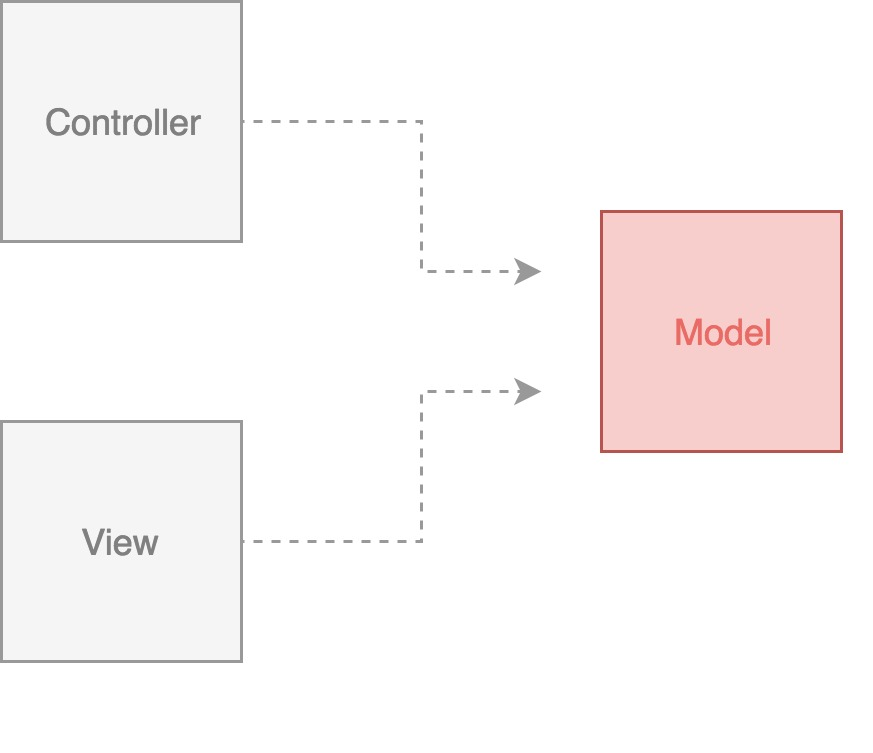
\includegraphics[width=5.5cm]{./images/MVCdefault}
\caption{Architettura MVC classica.}
\label{MVCdefault}
\end{wrapfigure}

Il Model rappresenta i dati che formano tutta o una parte dello stato dell'applicazione e come essi mutano. E' possibile immaginare questo componente come un oggetto che identifica un elemento specifico del servizio e ne descrive come il suo stato muta ad una eventuale azione. Il Model è “cieco", nel senso che tutto ciò che fa è mantenere dati e descrivere come essi cambiano, non avendo in alcun modo né la possibilità di conoscere in che modo influenzano l'applicazione né la capacità autonoma di effettuare modifiche su di essi se non sotto specifica istruzione del Controller.

I componenti che compongono la View hanno l'obiettivo di rappresentare i dati del Model in una forma facilmente comprensibile all'utente finale. Nell'architettura standard MVC il ruolo della View era piuttosto dinamico e organizzava i suoi aggiornamenti discutendo direttamente con il Model ed ottenendo i dati da esso, lasciando al Controller il compito di gestire gli input dell'utente. In questo modo l'architettura era organizzata con il Model come componente centrale togliendo importanza al Controller.

Andando avanti nel tempo e con la comparsa sempre più frequente più framework ispirati a questo pattern, l'evoluzione ha cambiato leggermente le regole standard dettando che la View dovrebbe avere il meno possibile un ruolo “attivo" di lettura degli aggiornamenti del Model, e che la gran parte delle informazioni dovrebbe passare attraverso il Controller che diventa così l'elemento principale addetto alla logica \cite{HopkinsOnMVCandPHP}.

\begin{wrapfigure}{l}{7cm}
\centering 
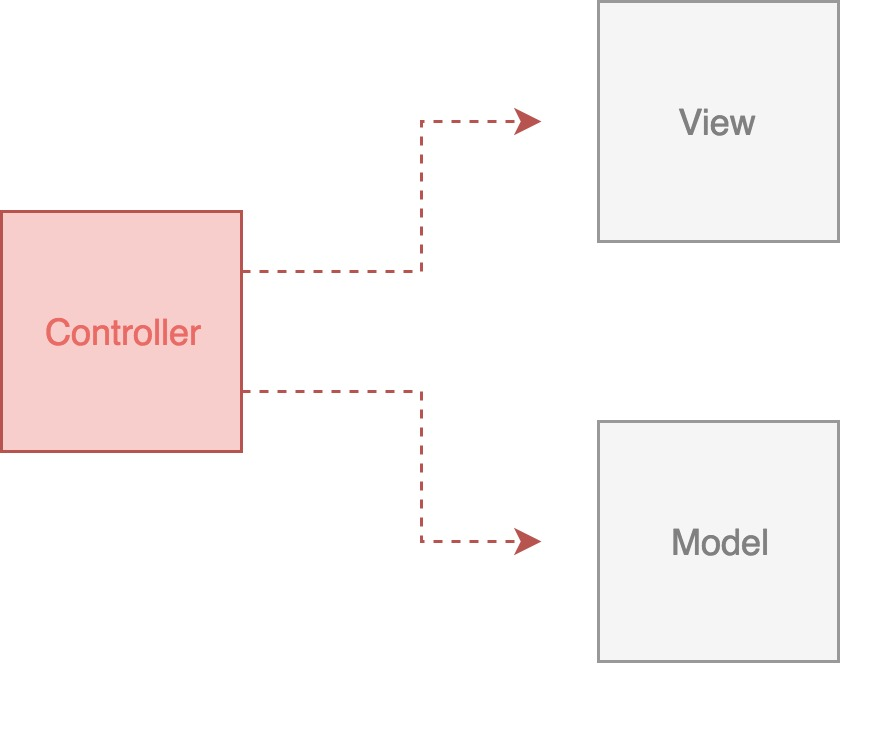
\includegraphics[width=5.5cm]{./images/MVCpassiveview}
\caption{Architettura MVC recente.}
\label{MVCpassiveview}
\end{wrapfigure}

Il Controller, nella versione classica dell'architettura MVC, si occupa solo ed esclusivamente di gestire gli input forniti dall'utente, trasmettendo le informazioni ricevute al Model. E' bene tenere presente che ogni Controller viene eseguito solamente a seguito di una azione che l'utente ha intrapreso dalla View e che quest'ultima ha un collegamento diretto con il Model comunicando attraverso il pattern Observer per adeguarsi ai vari cambiamenti dello stato.
Nelle versioni più recenti dell'architettura MVC invece, il Controller assume sempre di più la parte centrale incaricata di organizzare e collegare le altre due (Figura \ref{MVCpassiveview}). Non solo si occupa di gestire i vari eventi ed input generati dall'utente, ma si occupa anche di fornire e filtrare i dati del Model alla View, sottolineando la loro natura in questo caso più statica.

\section{MVC nel front-end}
L'architettura MVC è nata per risolvere il problema dell'organizzazione e della struttura del codice in applicazioni desktop scritte in Smalltalk-80. La sua versatilità e potenza ha tuttavia fatto sì che anche tutt'ora questo paradigma venga utilizzato nella stragrande maggioranza delle applicazioni, specialmente lato back-end.
Con la nascita delle SPA e con lo spostamento della logica sempre più verso il front-end tuttavia si sono presentati diversi problemi con l'architettura MVC classica i quali hanno spinto quest'ultima a modificarsi ed adattarsi al nuovo ambiente.

Lato front-end l'architettura MVC assume diverse forme a seconda del tipo di caratteristiche di cui abbiamo bisogno. Molti framework in Javascript tentano di includere il lavoro del Controller all'interno della View, altri al contrario rendono quest'ultima completamente passiva spostando tutta la logica al Controller, altri ancora aggiungono semplicemente nuovi livelli di divisione. Queste differenti architetture derivate vengono associate ad una macro-categoria chiamata \textit{MV*} (l'asterisco al posto della “C" di Controller sta a significare che questo è l'elemento che viene solitamente sostituito o modificato) dalla quale è possibile estrapolare due tra i più famosi ed utilizzati paradigmi lato front-end: MVP e MVVM \cite{OsmaniOnJSFrameworks}.

\subsection{MVP}
\label{ThesisMVPSection}
L'architettura MVP nasceva nel 1990 nell'azienda Talingent e veniva utilizzata per lo sviluppo di applicazioni in C++ e Java \cite{Potel1996mvp}. E' stata successivamente ripresa da vari framework Javascript tra cui uno dei più famosi è sicuramente Backbone.js.

Mentre nella versione classica di MVC, la View osservava il Model e si modificava di conseguenza, l'evoluzione di questo pattern ha fatto sì che il ruolo di osservatore passasse sempre più al Controller, ora chiamato Presenter, che costituisce un vero e proprio elemento centrale ed intermediario, eliminando quindi completamente la logica dalla View (Figura \ref{MVPworkflow}).

\begin{figure}[h]
\centering 
\vspace*{0.5cm}
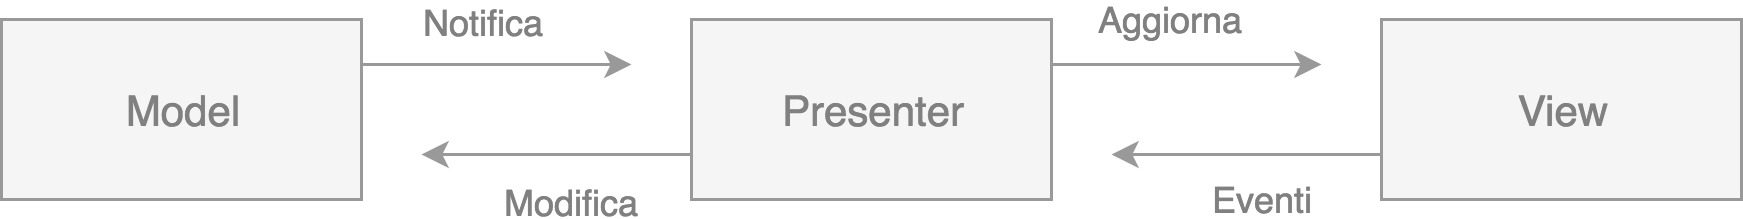
\includegraphics[width=13cm]{./images/MVPworkflow}
\caption{Architettura MVP.}
\label{MVPworkflow}
\vspace*{0.5cm} 
\end{figure}

MVP è un paradigma utilizzato specialmente per applicazioni a livello enterprise, con View complesse e grandi quantità di interazioni da parte dell'utente in quanto tutta la logica risiede nel Presenter rendendo l'applicazione semplice da testare e staccando la View dal resto rendendola particolarmente riutilizzabile all'interno del codice.
Tuttavia le differenze tra le architetture MVC e MVP sono solo a livello semantico, interpretando cioè diversamente un componente comune ad entrambe. Molti problemi più radicati che troviamo nella prima quindi si vengono comunque a presentare nella seconda \cite{OsmaniOnJSFrameworks}.

\subsection{MVVM}
L'architettura MVVM è stata per prima definita da Microsoft in un post del 2005 di John Grossman \cite{GossmanOnMVVM}. E' nata come una architettura per la creazione di applicazioni con Windows Presentation Foundation (WPF) ed è stata successivamente implementata con un discreto successo in framework Javascript come Knockout.js\footnote{http://knockoutjs.com}.

Questo paradigma si basa completamente sulla sincronizzazione della View attraverso il pattern Observer. La logica dell'applicazione quindi questa volta è posizionata quasi interamente nella View e, mentre il Model si comporta come da norma solamente da “memoria", questa ne osserva i cambiamenti e si aggiorna di conseguenza. La vera differenza è che in questo caso le azioni dell'utente sono gestite direttamente dalla View, in quanto il vincolo posto sui dati è bidirezionale (modificando l'elemento in input nella View viene automaticamente modificato il valore referenziato).

\begin{figure}[h]
\centering 
\vspace*{0.5cm}

\includegraphics[width=13cm]{./images/MVVMworkflow}
\caption{Architettura MVVM.}
\label{MVVMworkflow}
\vspace*{0.5cm} 
\end{figure}

La View tuttavia non può leggere direttamente i dati di cui ha bisogno dal Model, i quali nella maggior parte dei casi sono grezzi e hanno bisogno di essere filtrati e lavorati. Per questo è stato creato un nuovo componente, che sostituisce il Controller, chiamato ViewModel (Figura \ref{MVVMworkflow}) il quale si pone come livello passivo intermedio tra Model e View, ed estrapola i dati utili dal primo e li rende disponibili in maniera comprensibile al secondo, oltre anche a fornire funzioni utili alla gestione dello stato e degli eventi \cite{OsmaniOnJSFrameworks}.

Uno dei punti forti dell'architettura MVVM implementata dai più recenti framework Javascript riguarda l'astrazione della View per l'utilizzo dei vincoli di dati bidirezionali (anche chiamati \textit{Two-ways data bindings}) del ViewModel direttamente all'interno del DOM (Codice \ref{exampleMVVMDataBinding}).

\begin{listing}[ht]
\inputminted{jsx}{sources/exampleMVVMDataBinding.js}
\caption{Esempio di vincolo di dati nel DOM.}
\label{exampleMVVMDataBinding}
\end{listing}

Da una parte questi facilitano enormemente l'implementazione dell'interfaccia e consentono di ridurre in maniera considerevole la logica da implementare a parte all'interno del ViewModel, dall'altra sono considerati un tipo di programmazione obsoleta che mischia la logica con il linguaggio di markup.

\section{Il flusso dei dati}
MVC, insieme alle sue architetture derivate, è un paradigma nel quale il flusso di dati avviene in maniera bidirezionale. L'utente esegue un'azione dalla View, che viene interpretata ed eseguita dalla relativa sezione dove risiede la logica dell'interfaccia (ad esempio quindi dal Controller se si parla di MVC classico o dal Presenter nel MVP) la quale apporterà le dovute modifiche ai dati presenti all'interno del Model causando una notifica da parte di quest'ultimo a tutti gli altri componenti della View segnalando l'avvenuto cambiamento. Il flusso, come possiamo vedere nell'immagine \ref{MVPworkflow}, avviene quindi sia dal Model alla View che vice versa.

\subsection{Analisi dell'applicazione}
\label{ExampleApplicationMVC}
Per analizzare più in dettaglio ciò che è stato appena descritto, verrà utilizzata una applicazione esempio fine a se stessa costruita utilizzando il framework \textit{Backbone.js} e quindi l'architettura MVP. Tutte le affermazioni che verranno fatte tuttavia non riguarderanno solo ed esclusivamente questa architettura, ma si estenderanno anche alle altre derivate da MVC, in quando descriveranno problematiche radicate nel paradigma.

\begin{figure}[h]
\centering
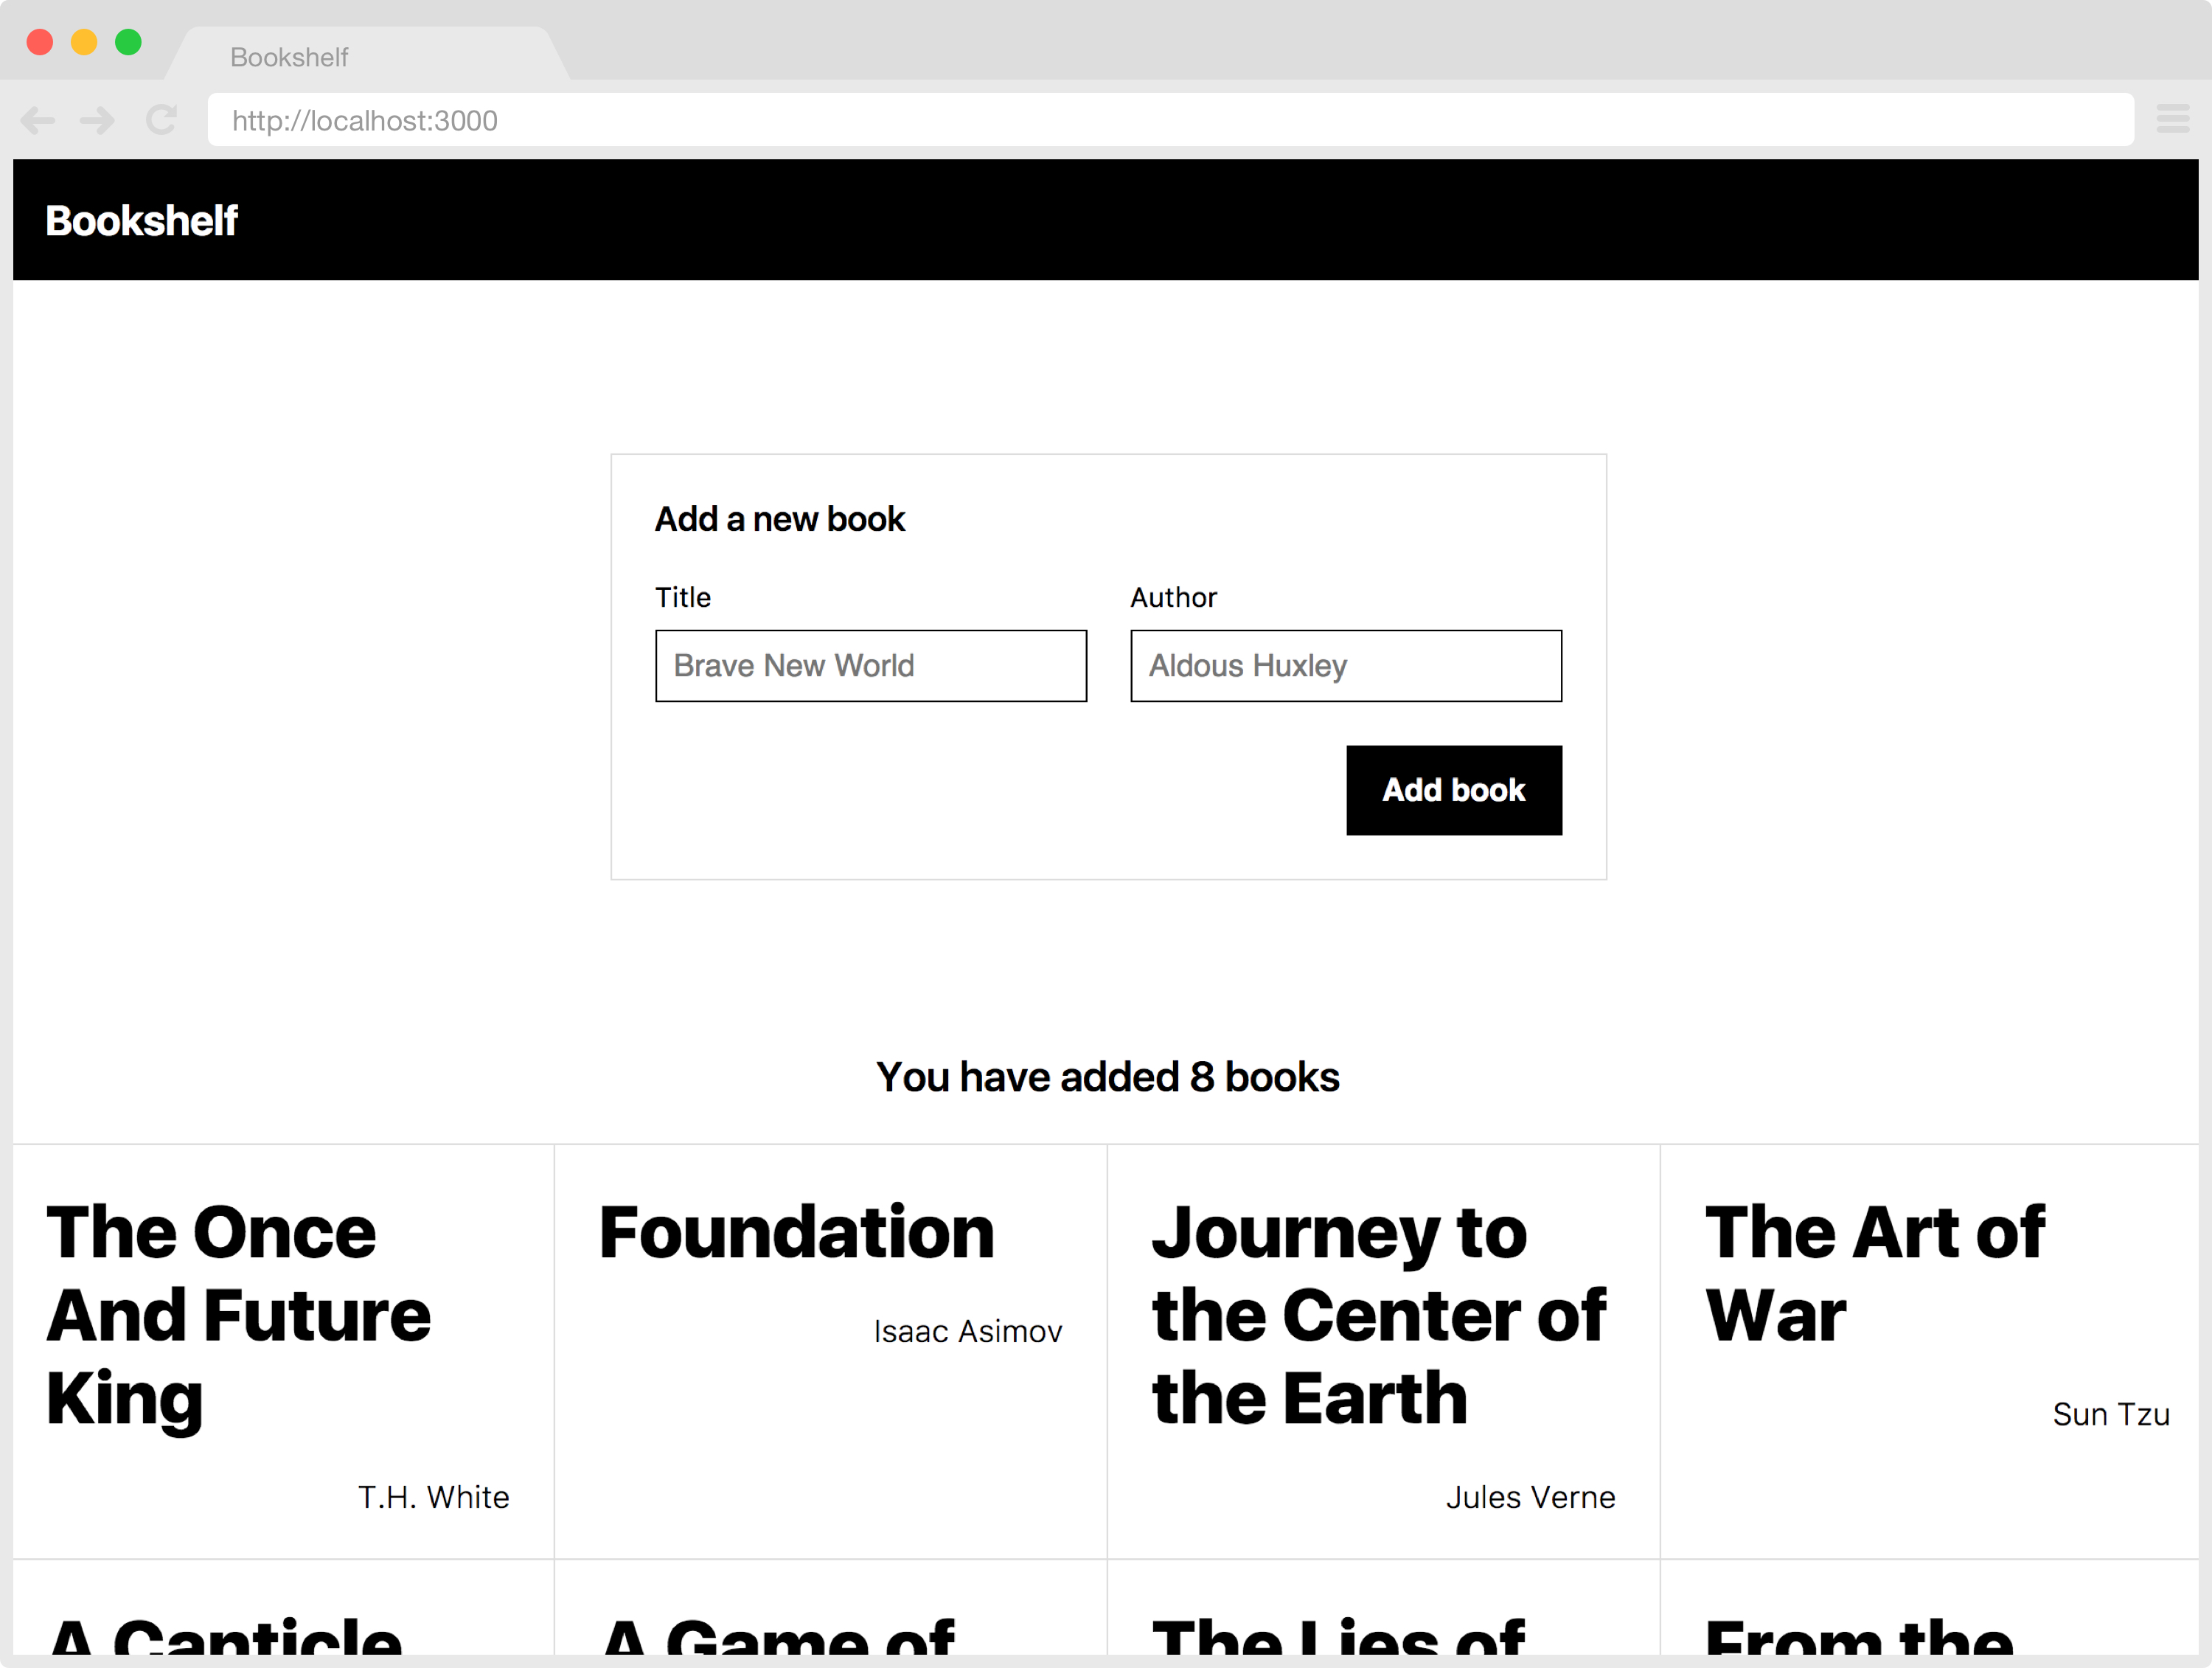
\includegraphics[width=14cm]{./images/bookshelfApplication1}
\caption{Applicatione esempio per un database di libri.}
\label{bookshelfApplication1}
\end{figure}

L'applicazione\footnote{Codice completo a https://github.com/diegopq/unicam-thesis-examples.} nella Figura \ref{bookshelfApplication1} rappresenta un semplice database di libri con la possibilità di aggiungerne di nuovi tramite il form in alto, ed eliminare quelli presenti andando con il mouse sopra un libro e cliccando alla comparsa del simbolo “×".
Il codice è scritto utilizzando la sintassi e il sistema di moduli di ES6 usando Webpack con Babel (in coppia con il plugin \textit{Env preset}\footnote{https://babeljs.io/docs/plugins/preset-env}, utilizzato per determinare automaticamente la versione di ES utilizzata) per creare il file Javascript compilato e completo di dipendenze. Anche il CSS per comodità è stato aggiunto nel pacchetto ed automaticamente applicato alla pagina dell'applicazione attraverso i loaders \textit{css-loader}\footnote{https://github.com/webpack-contrib/style-loader} e \textit{style-loader}\footnote{https://github.com/webpack-contrib/css-loader}.
Le uniche due dipendenze richieste da \textit{Backbone.js} consistono in: \textit{jQuery}\footnote{https://jquery.com/}, libreria per la manipolazione del DOM che mette a disposizione altre utili funzioni come animazioni, gestione degli eventi e chiamate Ajax; \textit{Underscore.js}\footnote{http://underscorejs.org/}, una raccolta di metodi per gestione di oggetti, array e collezioni varie attraverso tecniche utilizzate nel paradigma di programmazione funzionale.

Di seguito verranno analizzate le sezioni fondamentali dell'applicazione con le relative parti di codice più importanti per capire come questo framework riesca a gestire la problematica del flusso di dati.

\subsubsection*{Model}
Il Model di una applicazione scritta con \textit{Backbone.js} è un oggetto che estende \mintinline{text}{Backbone.Model} e che racchiude dentro di sé dei dati strutturati. Nel caso dell'applicazione presentata, il Model più basilare descrive lo stato di un singolo libro che è composto da due parametri: “title" e “author", dando loro un valore di default (Codice \ref{applicationMVCModel}).

\begin{listing}[ht]
\inputminted{Javascript}{sources/applicationMVCBookModel.js}
\caption{Model dell'applicazione relativo ad un libro.} 
\label{applicationMVCModel} 
\end{listing}

Il modo definitivo per descrivere lo stato dell'applicazione tuttavia è attraverso una lista di libri. È necessario quindi creare un tipo di Model che rappresenti questo concetto in maniera opportuna. \textit{Backbone.js} mette a disposizione la classe \mintinline{text}{Backbone.Collection} che rappresenta esattamente una “collezione di Model" e gestisce in maniera automatica tutti gli elementi al suo interno riconoscendo come istanza di \mintinline{text}{BookModel} qualsiasi elemento aggiunto ad essa (Codice \ref{applicationMVCBookCollection}).

\begin{listing}[ht]
\inputminted{Javascript}{sources/applicationMVCBookshelfCollection.js}
\caption{Model dell'applicazione relativo ad una lista di libri.} 
\label{applicationMVCBookCollection} 
\end{listing}

La classe Collection è implementata come se fosse una normale collezione di elementi (o lista) e \textit{Backbone.js} ci mette a disposizione tutti i metodi per interagire con essa. 
Ogni qualvolta questa lista o un suo elemento viene modificato, la stessa si occupa di propagare il corrispettivo evento a tutte le View ad essa collegate in modo da permettere loro di aggiornarsi di conseguenza.
Viene poi creata un'istanza di questa collezione, popolata con dei libri di default letti dal file JSON \mintinline{text}{db.json} ed esportata ottenendo così un Singleton\footnote{Il “Singleton” è un design pattern che restringe ad uno il numero massimo di istanze che una classe può avere. E' utilizzato molto spesso quando c'è bisogno di avere un oggetto condiviso globalmente all'interno di una applicazione.} che rappresenta l'intero stato dell'applicazione condiviso globalmente tra tutti i componenti.

\subsubsection*{View}
Una View in \textit{Backbone.js} corrisponde al codice HTML dell'applicazione (Codice \ref{applicationMVCView}). Oltre che gestire questo, tuttavia, permette di definire dei piccoli “modelli” all'interno di un tag \mintinline{text}{<script type='text/template'>} che verranno poi popolati in modo dinamico attraverso un \textit{Template engine}, ossia una libreria che combina un template con un modello di dati, come ad esempio \textit{Mustache}\footnote{https://mustache.github.io} o \textit{EJS}\footnote{http://ejs.co}.

In questa applicazione viene utilizzato \textit{Underscore.js}, che è già una dipendenza di default dell'applicazione e mette a disposizione un piccolo sistema di templating basilare.

\begin{listing}[ht]
\inputminted{xml}{sources/applicationMVCView.html}
\caption{Templates dell'applicazione.} 
\label{applicationMVCView} 
\end{listing}

\subsubsection*{Presenter}
L'oggetto che estende \mintinline{text}{Backbone.View} è il componente centrale di \text{Backbone.js} e rappresenta il Presenter nell'architettura MVP. Ha un ruolo centrale sia all'interno dell'applicazione per le sue innumerevoli funzioni, sia nell'architettura in quanto si pone tra gli altri due componenti e li coordina in maniera attiva.

\begin{listing}[ht]
\inputminted{javascript}{sources/applicationMVCPresenter.js}
\caption{Presenter dell'applicazione.} 
\label{applicationMVCPresenter} 
\end{listing}

La classe \mintinline{text}{Backbone.View} rappresenta, in pratica, un elemento che verrà poi aggiunto al DOM dell'applicazione tramite il metodo \mintinline{text}{render()}. Il tipo di elemento e le sue classi sono descritte attraverso le proprietà \mintinline{text}{tagName} e \mintinline{text}{className}.
Il contenuto invece viene definito in principio all'interno della stessa funzione \mintinline{text}{render}, e nel caso del Codice \ref{applicationMVCPresenter} viene utilizzato il template engine messo a disposizione da \textit{Underscore.js} per popolare il template selezionato.
La gestione degli eventi è uno dei compiti più delicati del Presenter. Esistono due tipi di eventi da gestire:

\begin{itemize}
    \item \textbf{Eventi dal Model}: sono quegli eventi che partono dal Model a seguito di una modifica di quest'ultimo (l'aggiunta o la modifica di un elemento all'interno di una collezione).
    \item \textbf{Eventi dalla View}: sono quegli eventi che vengono innescati da un certo comportamento dell'utente che utilizza la View dell'applicazione (il click di un pulsante o la scrittura all'interno di un campo di testo).
\end{itemize}

Gli eventi del primo tipo vengono gestiti all'interno del metodo \mintinline{text}{initialize()}, attraverso la funzione \mintinline{text}{View.listenTo()} passando ad essa il Model o la Collection da osservare (è possibile utilizzare \mintinline{text}{this.collection} o \mintinline{text}{this.model} a seconda del tipo di Model assegnato alla View al suo avvio), il tipo di evento e la relativa funzione che dovrà essere eseguita.
Per la gestione degli eventi che provengono dalla View invece si utilizza l'oggetto \mintinline{text}{events} specificando il tipo di evento da controllare, il selettore per identificare l'elemento vincolato nel DOM e la funzione da chiamare all'innesco dell'evento (Codice \ref{applicationMVCPresenterEvents}). \textit{Backbone.js} si occuperà poi di assegnare e gestire questi eventi a ciascun elemento del DOM selezionato, risolvendo anche il classico problema di assegnare eventi ad elementi creati successivamente in maniera dinamica.

\begin{listing}[ht]
\inputminted{javascript}{sources/applicationMVCPresenterEvents.js}
\caption{Presenter con la gestione degli eventi dalla View.} 
\label{applicationMVCPresenterEvents} 
\end{listing} 

\subsection{Effetto cascata}
Come presentato nei capitoli precedenti, MVC è un'ottima architettura per strutturare il codice, tuttavia soffre di problemi non indifferenti quando utilizzata lato front-end ed in applicazioni di una certa complessità.

\begin{figure}[h]
\centering
%\vspace*{0.5cm} 
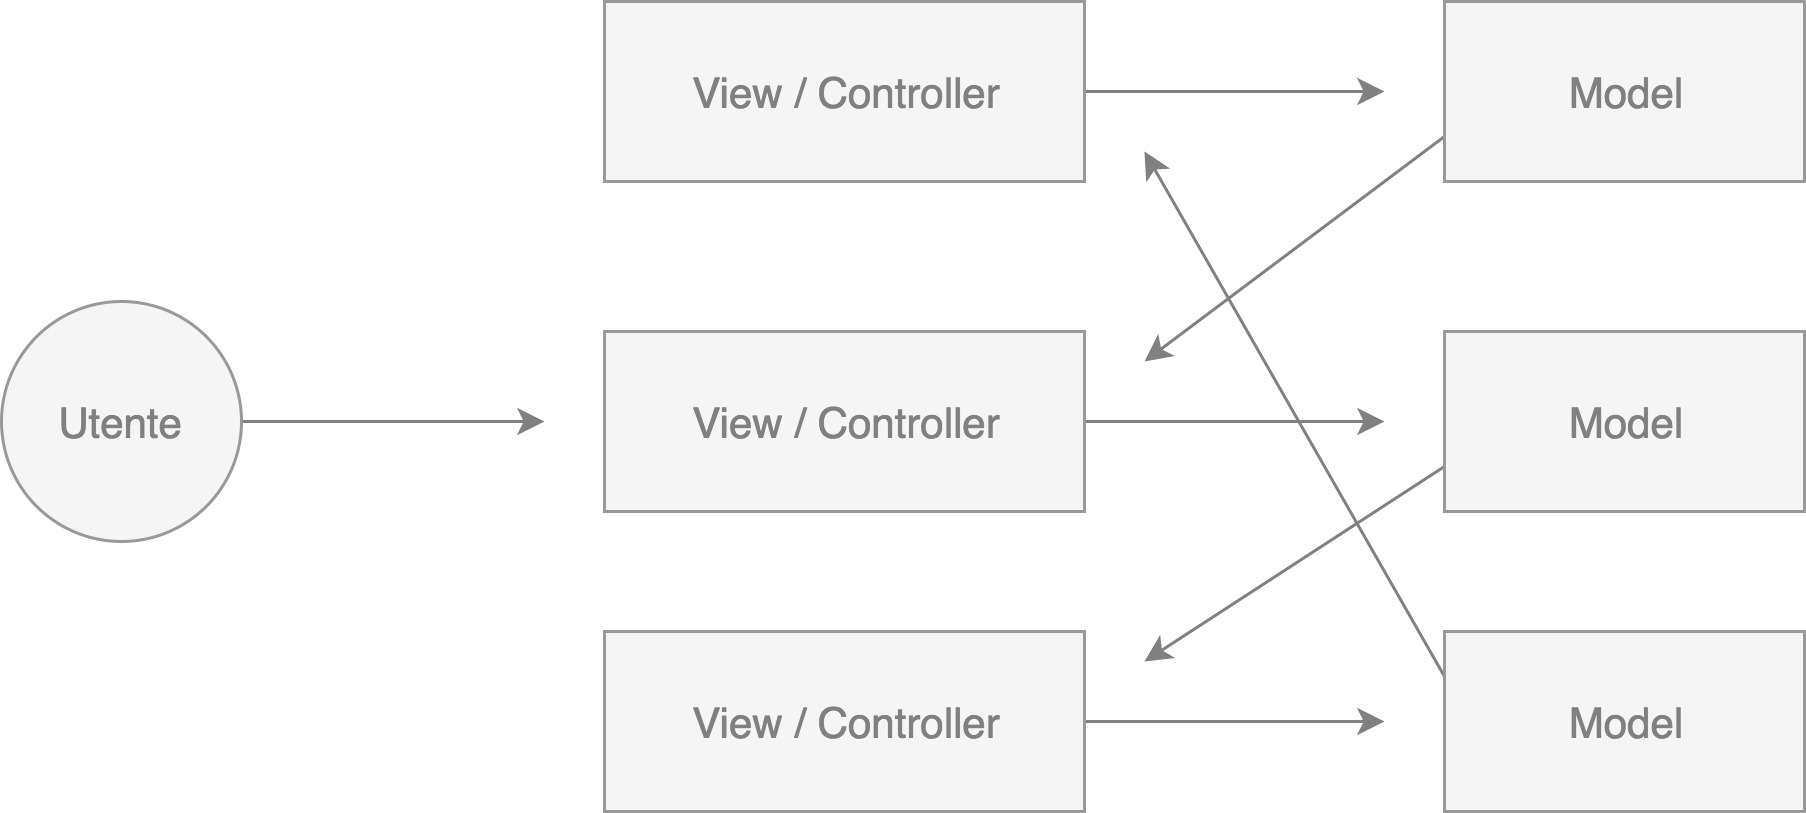
\includegraphics[width=12cm]{./images/MVCDataFlow}
\caption{Rappresentazione del flusso di dati in un'architettura MVC.}
\label{MVCDataFlow}ì
%\vspace*{0.5cm}
\end{figure}

L'esempio riportato nella Figura \ref{MVCDataFlow} rappresenta il tallone d'Achille di questo paradigma (e dei suoi derivati). Un'azione scaturita dall'utente, innesca un evento nel Controller (o qualsiasi altro componente che si occupa di gestire gli eventi) il quale apporta le opportune modifiche al Model, che a sua volta notifica gli altri componenti dell'aggiornamento avvenuto facendo scaturire nuovi eventi e nuove modifiche. Questo comportamento viene chiamato “Cascading effect” e causa estrema difficolta nel debugging del codice specialmente per quanto riguarda l'analisi degli effetti che un evento causa all'applicazione.

Un pratico esempio di questo problema è spiegato dai programmatori di Facebook, e descrive la relazione tra chat e notifiche. Quando abbiamo una chat aperta ed arriva un messaggio, questo viene riportato all'interno della chat, e sotto forma di nuova notifica. La chat e le notifiche sono due View separate che però prendono i dati da uno stesso Model. Quando si effettua un click sulla chat la notifica viene automaticamente letta, come anche vice versa se si clicca sulla notifica comparirà il simbolo di “messaggio visualizzato” nella chat.
All'interno dei rispettivi Controller questi comportamenti devono essere sincronizzati ed applicati in maniera corretta tenendo presente lo stato di ciascun altro elemento e tutte le varie eccezioni che possono incorrere. Tutto ciò rende difficile scalare l'applicazione aggiungendo nuove features collegate \cite{JingChenOnMVCAndFlux}.